%==========================
% Chapter 8: Variational Inference, Bits-Back, and Flows
%==========================

\chapter{Variational Inference, Bits-Back, and Flows}
\label{ch:vae_flows}

\vspace{1em}

In the previous chapters, we explored models that generate data in different ways: transformers build sequences one token at a time, diffusion models gradually denoise pure noise into structured samples. Now we turn to another fundamental approach: models that learn a compressed latent representation of data. Imagine being asked to describe a photograph using only ten numbers. Those ten numbers are a bottleneck, forcing you to capture only the most essential features: perhaps the overall scene type, the dominant colors, the spatial layout. This is the core idea behind variational autoencoders.

\vspace{0.3cm}

But there is a deeper connection here. In Chapter 7, we derived the evidence lower bound for diffusion models and saw that maximizing likelihood requires balancing reconstruction quality against prior matching. That same mathematical structure appears whenever we have latent variables. The ELBO is not just a training objective for one model family; it is a fundamental theorem about how information must be allocated when compressing data through hidden representations.

\vspace{0.3cm}

This chapter surveys the space of latent variable models through three lenses. First, we will see how variational inference turns posterior approximation into a compression problem, where the ELBO measures codelength. Second, we will explore bits-back coding, which reveals why the ELBO is exactly the right objective by showing how to build an optimal compressor from a variational model. Third, we will study normalizing flows, which avoid approximation altogether by learning invertible transformations with exact likelihoods. Along the way, we will connect these ideas to language modeling, understand when each approach excels, and develop geometric intuitions about what these models are really doing in probability space.

\vspace{2em}

%==========================
\section{The Variational Framework: Approximating Intractable Posteriors}
\label{sec:variational_framework}
%==========================

\vspace{1em}

\subsection{The Problem: Exact Inference is Intractable}

Suppose we have observed data $x$ and believe it was generated from some latent variable $z$ through a process we model as $p_\theta(x \mid z)$. The latent variable might represent semantic content (what is in an image), discrete structure (parse trees in language), or continuous factors (temperature and pressure in physics). To make predictions or generate new data, we need the posterior distribution $p_\theta(z \mid x)$, which tells us what latent states are consistent with the observed data.

\vspace{0.3cm}

By Bayes' rule, the posterior is:
%
\begin{equation}
p_\theta(z \mid x) = \frac{p_\theta(x \mid z) p_\theta(z)}{p_\theta(x)}
= \frac{p_\theta(x \mid z) p_\theta(z)}{\int p_\theta(x \mid z') p_\theta(z') \, dz'}
\end{equation}

\vspace{0.3cm}

The numerator is easy to compute: we chose the prior $p_\theta(z)$ and likelihood $p_\theta(x \mid z)$ to be tractable. But the denominator, called the evidence or marginal likelihood, requires integrating over all possible latent values. For continuous $z$ in high dimensions, this integral is almost always intractable. For discrete $z$ with combinatorial structure, the sum is exponentially large.

\vspace{0.3cm}

This is not a minor technical obstacle. It is a fundamental barrier. If we cannot compute $p_\theta(z \mid x)$, we cannot sample from it, we cannot optimize model parameters using exact gradients, and we cannot even evaluate how well our model explains the data. We need a way forward.

\vspace{1.5em}

\begin{pausebox}
\textbf{Pause and Reflect.} Think about a simple example: fitting a Gaussian mixture model to data. You have latent cluster assignments $z$ and want to know which cluster each data point belongs to. The posterior $p(z \mid x)$ depends on all the mixture weights and cluster parameters. Even with just ten clusters, computing the posterior exactly requires considering how each point's assignment affects every other point's assignment through the shared parameters. The combinatorics explode quickly.
\end{pausebox}

\vspace{1.5em}

\subsection{The Variational Solution: Approximate with a Simpler Family}

Variational inference sidesteps exact computation by approximating the posterior with a tractable distribution $q_\phi(z \mid x)$ from some chosen family. The word "variational" here means we are turning inference into an optimization problem: we vary the parameters $\phi$ to make $q_\phi$ as close as possible to the true posterior $p_\theta(z \mid x)$.

\vspace{0.3cm}

How do we measure closeness? The natural choice is the Kullback-Leibler divergence:
%
\begin{equation}
D_{\text{KL}}(q_\phi(z \mid x) \| p_\theta(z \mid x))
= \mathbb{E}_{q_\phi} \left[ \log \frac{q_\phi(z \mid x)}{p_\theta(z \mid x)} \right]
\end{equation}

\vspace{0.3cm}

We want to minimize this divergence, making $q_\phi$ a good approximation. But there is a problem: computing this KL divergence requires knowing $p_\theta(z \mid x)$, which is exactly what we do not have. It seems we are stuck in a circular dependency.

\vspace{0.3cm}

The breakthrough insight is that we can rearrange this divergence to derive a quantity that does not require the posterior. Start by expanding the KL using the definition of the posterior:
%
\begin{align}
D_{\text{KL}}(q_\phi(z \mid x) \| p_\theta(z \mid x))
&= \mathbb{E}_{q_\phi} \left[ \log q_\phi(z \mid x) - \log p_\theta(z \mid x) \right] \\
&= \mathbb{E}_{q_\phi} \left[ \log q_\phi(z \mid x) - \log p_\theta(x, z) + \log p_\theta(x) \right] \\
&= \mathbb{E}_{q_\phi} \left[ \log q_\phi(z \mid x) - \log p_\theta(x, z) \right] + \log p_\theta(x)
\end{align}

\vspace{0.3cm}

Rearranging, we get:
%
\begin{equation}
\log p_\theta(x) = \mathbb{E}_{q_\phi} \left[ \log p_\theta(x, z) - \log q_\phi(z \mid x) \right] + D_{\text{KL}}(q_\phi(z \mid x) \| p_\theta(z \mid x))
\end{equation}

\vspace{0.3cm}

The first term on the right is called the evidence lower bound, or ELBO:
%
\begin{equation}
\text{ELBO}(q_\phi, \theta; x) = \mathbb{E}_{q_\phi} \left[ \log p_\theta(x, z) - \log q_\phi(z \mid x) \right]
\end{equation}

\vspace{0.3cm}

Since the KL divergence is always non-negative, we have:
%
\begin{equation}
\log p_\theta(x) \geq \text{ELBO}(q_\phi, \theta; x)
\end{equation}

\vspace{0.3cm}

This is the fundamental inequality. The ELBO lower-bounds the log-evidence. When $q_\phi(z \mid x) = p_\theta(z \mid x)$, the KL is zero and the bound is tight. Otherwise, there is a gap equal to the KL divergence between our approximation and the true posterior.

\vspace{1.5em}

\begin{figure}[t]
\centering
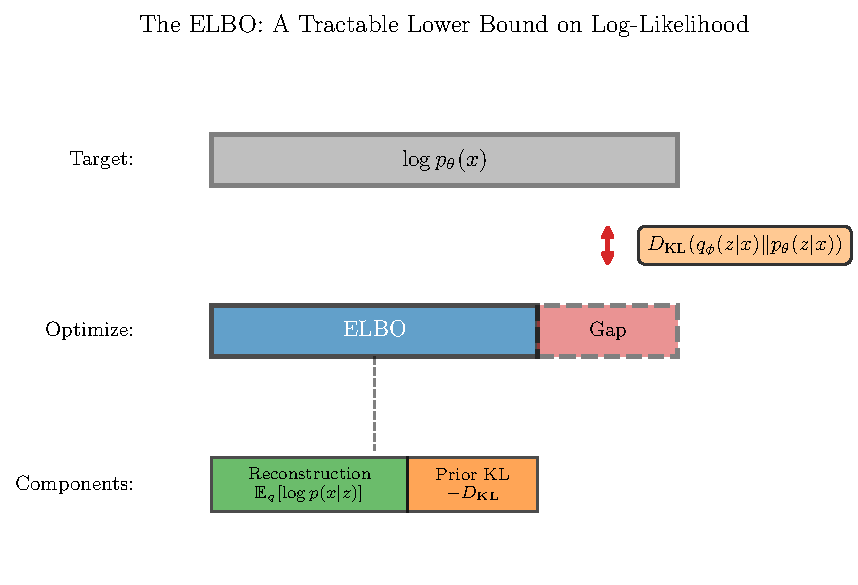
\includegraphics[width=\linewidth]{code/figures/ch08_variational_flows/fig_8_1_elbo_decomposition.pdf}
\caption{Variational inference trades off reconstruction accuracy against posterior regularization: the ELBO lower-bounds $\log p_\theta(x)$ with a gap equal to the KL divergence between $q_\phi(z\mid x)$ and the true posterior.}
\label{fig:elbo_bound_gap}
\end{figure}

\vspace{1.5em}

\begin{keyinsight}
The ELBO is a tractable surrogate for log-likelihood. We can compute it using only the prior $p_\theta(z)$, the likelihood $p_\theta(x \mid z)$, and our approximate posterior $q_\phi(z \mid x)$, all of which we designed to be tractable. Maximizing the ELBO with respect to $\phi$ minimizes the KL divergence to the true posterior, giving us the best approximation within our chosen family.
\end{keyinsight}

\vspace{1.5em}

\subsection{Decomposing the ELBO: Reconstruction and Regularization}

The ELBO can be rewritten in a more intuitive form by expanding the joint distribution:
%
\begin{align}
\text{ELBO}(q_\phi, \theta; x)
&= \mathbb{E}_{q_\phi} \left[ \log p_\theta(x \mid z) + \log p_\theta(z) - \log q_\phi(z \mid x) \right] \\
&= \mathbb{E}_{q_\phi} \left[ \log p_\theta(x \mid z) \right] - D_{\text{KL}}(q_\phi(z \mid x) \| p_\theta(z))
\end{align}

\begin{keyinsight}
\textbf{Two-part MDL (Chapter~1) callback.} The ELBO has the exact structure of a two-part Minimum Description Length code. The term $-\log p_\theta(z)$ pays to specify \emph{which latent code} (model part), while $-\log p_\theta(x\mid z)$ pays to transmit the data given that code (data part). Taking expectations under $q_\phi(z\mid x)$ yields the familiar \emph{KL rate} plus \emph{reconstruction distortion}. This is the same decomposition introduced in Chapter~1's two-part codes, now instantiated by a learned latent representation.
\end{keyinsight}

\vspace{0.3cm}


\vspace{0.3cm}

This decomposition reveals two competing objectives. The first term, $\mathbb{E}_{q_\phi}[\log p_\theta(x \mid z)]$, is the reconstruction term. It measures how well we can decode $x$ from latent codes sampled from $q_\phi$. To maximize this term, the decoder should be expressive and the posterior should put probability mass on latent codes that explain $x$ well.

\vspace{0.3cm}

The second term, $-D_{\text{KL}}(q_\phi(z \mid x) \| p_\theta(z))$, is the regularization term. It penalizes approximate posteriors that deviate from the prior. To maximize this term (minimize the KL), $q_\phi(z \mid x)$ should stay close to $p_\theta(z)$.

\vspace{0.3cm}

These two objectives are in tension. If we make $q_\phi(z \mid x)$ very flexible and far from the prior, we can achieve better reconstruction but pay a KL penalty. If we force $q_\phi(z \mid x) \approx p_\theta(z)$, we minimize the KL but may sacrifice reconstruction quality. The ELBO finds the optimal balance.

\vspace{1.5em}

\begin{figure}[t]
\centering
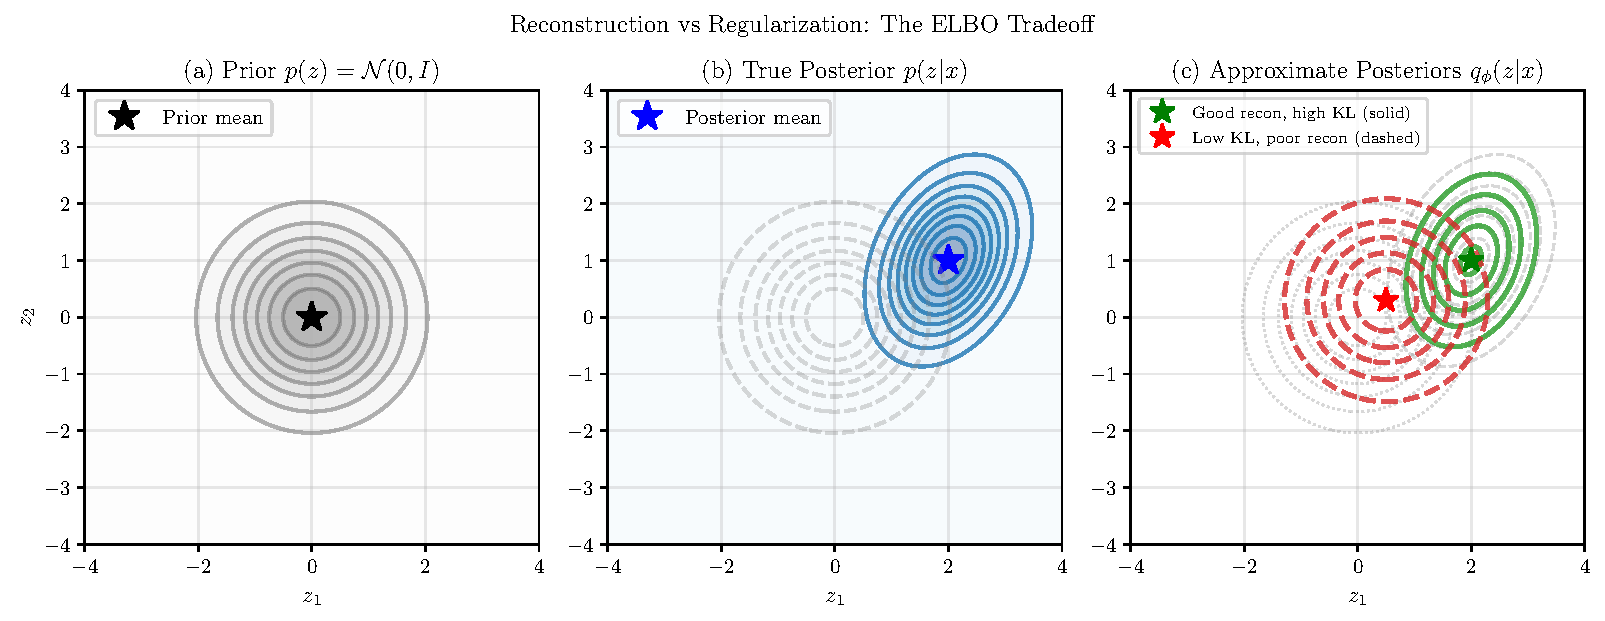
\includegraphics[width=\linewidth]{code/figures/ch08_variational_flows/fig_8_2_recon_regularization.pdf}
\caption{Reconstruction fidelity and posterior regularization pull in opposite directions; the ELBO balances them along a rate--distortion frontier.}
\label{fig:recon_regularization_tradeoff}
\end{figure}

\vspace{1.5em}

\begin{geometrylens}
From an information geometry perspective, the ELBO decomposition separates two projections. The reconstruction term pulls the posterior toward regions of latent space that decode well, measured in the geometry of the likelihood manifold. The KL term pulls the posterior back toward the prior, measured in the geometry of the latent space. The optimal posterior lives at the intersection of these two constraints, balancing explanatory power against simplicity.
\end{geometrylens}

\vspace{1.5em}

\subsection{The Reparameterization Trick: Making Gradients Flow}

To train a variational autoencoder, we need to optimize the ELBO with respect to both the encoder parameters $\phi$ and the decoder parameters $\theta$. The gradient with respect to $\theta$ is straightforward because $\theta$ appears only inside the expectation. But the gradient with respect to $\phi$ is tricky: $\phi$ determines the distribution we are sampling from, so it affects both the integrand and the measure of integration.

\vspace{0.3cm}

The naive Monte Carlo gradient estimator is:
%
\begin{equation}
\nabla_\phi \text{ELBO} = \nabla_\phi \mathbb{E}_{q_\phi} [\log p_\theta(x, z) - \log q_\phi(z \mid x)]
\end{equation}

\paragraph{Geometric view (change of coordinates).}
Beyond the mechanics, it helps to see reparameterization as a \emph{coordinate change}. We move from the original latent coordinates $z$ to ``standard-noise'' coordinates $\epsilon$ in which the randomness is \emph{axis-aligned} and \emph{independent of $\phi$}. The deterministic map
%
\[
T_\phi(x, \epsilon) \;=\; \mu_\phi(x) \;+\; \sigma_\phi(x) \odot \epsilon
\]
%
then pushes $\epsilon \sim \mathcal{N}(0, I)$ forward to $z$. Gradients with respect to $\phi$ act only through $T_\phi$; the sampling measure no longer depends on $\phi$, which is why variance drops. In general, for any reparameterizable family we write $z = g_\phi(x, \epsilon)$ with a fixed base noise $\epsilon \sim p(\epsilon)$: we are \emph{choosing coordinates} where the stochasticity lives in $\epsilon$, and optimization over $\phi$ happens in the deterministic map $g_\phi$.

\vspace{0.3cm}


\vspace{0.3cm}

We cannot simply push the gradient inside the expectation because the expectation is over $q_\phi$, which depends on $\phi$. The score function estimator (also called REINFORCE) solves this by using the log-derivative trick, but it suffers from high variance.

\vspace{0.3cm}

The reparameterization trick provides a better solution for continuous latent variables. The key idea is to separate the randomness from the parameters. Instead of sampling $z \sim q_\phi(z \mid x)$ directly, we sample from a parameter-free noise distribution and transform it deterministically using $\phi$.

\vspace{0.3cm}

For a Gaussian posterior $q_\phi(z \mid x) = \mathcal{N}(\mu_\phi(x), \sigma^2_\phi(x))$, we can write:
%
\begin{equation}
z = \mu_\phi(x) + \sigma_\phi(x) \cdot \epsilon, \quad \epsilon \sim \mathcal{N}(0, I)
\end{equation}

\vspace{0.3cm}

Now $\epsilon$ does not depend on $\phi$, so we can rewrite the ELBO as:
%
\begin{equation}
\text{ELBO}(q_\phi, \theta; x) = \mathbb{E}_{\epsilon \sim \mathcal{N}(0,I)} \left[ \log p_\theta(x \mid \mu_\phi(x) + \sigma_\phi(x) \cdot \epsilon) \right]
- D_{\text{KL}}(q_\phi(z \mid x) \| p_\theta(z))
\end{equation}

\vspace{0.3cm}

The expectation is now over a fixed distribution, and the gradient can pass through $\mu_\phi$ and $\sigma_\phi$ using standard backpropagation. The KL term can often be computed in closed form (for example, when both $q_\phi$ and $p_\theta$ are Gaussians), avoiding any sampling at all for that term.

\vspace{1.5em}

\begin{figure}[t]
\centering
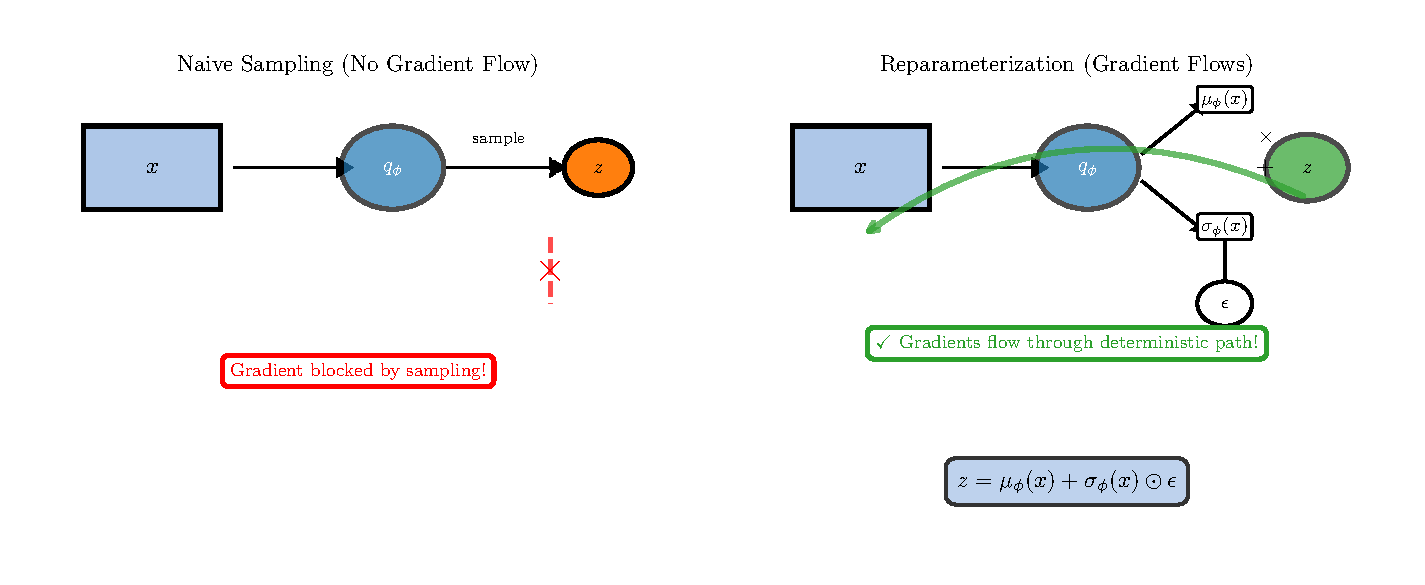
\includegraphics[width=\linewidth]{code/figures/ch08_variational_flows/fig_8_3_reparameterization.pdf}
\caption{The reparameterization trick isolates randomness in a base noise $\epsilon$ and pushes it through a differentiable map $g_\phi(x,\epsilon)$, enabling low-variance gradients for the ELBO.}
\label{fig:reparameterization}
\end{figure}

\vspace{1.5em}

\begin{examplebox}
\textbf{Worked Example: Gaussian VAE Gradient}

Suppose $p_\theta(z) = \mathcal{N}(0, I)$ and $q_\phi(z \mid x) = \mathcal{N}(\mu_\phi(x), \sigma^2_\phi(x) I)$. The KL divergence has a closed form:
%
\begin{equation*}
D_{\text{KL}}(q_\phi \| p_\theta) = \frac{1}{2} \sum_{j=1}^d \left( \sigma^2_{\phi,j}(x) + \mu^2_{\phi,j}(x) - 1 - \log \sigma^2_{\phi,j}(x) \right)
\end{equation*}

For the reconstruction term, sample $\epsilon \sim \mathcal{N}(0, I)$, compute $z = \mu_\phi(x) + \sigma_\phi(x) \cdot \epsilon$, then evaluate $\log p_\theta(x \mid z)$. The gradient $\nabla_\phi \log p_\theta(x \mid z)$ backpropagates through $\mu_\phi$ and $\sigma_\phi$ using the chain rule, treating $\epsilon$ as constant.

The combined gradient is:
%
\begin{equation*}
\nabla_\phi \text{ELBO} \approx \nabla_\phi \log p_\theta(x \mid z) - \nabla_\phi D_{\text{KL}}(q_\phi \| p_\theta)
\end{equation*}

where the second term has an exact gradient from the closed-form KL. This is the workhorse of VAE training.
\end{examplebox}

\vspace{2em}

%==========================
\vspace{1em}
\subsection{Rate--Distortion and $\beta$-VAE}
The ELBO is a rate--distortion objective: the \emph{rate} is $R= D_{\mathrm{KL}}(q(z\mid x)\,\|\,p(z))$ and the \emph{distortion} is $D = \mathbb{E}_{q}[{-}\log p(x\mid z)]$. $\beta$-VAE optimizes $-D-\beta R$, moving along the rate--distortion curve from Chapter~1.

\begin{keyinsight}
\textbf{Information bottleneck view.} The latent should carry only the information about $x$ that is useful for the task at hand. In Tishby et~al.'s \emph{Information Bottleneck} (IB), one seeks a representation $Z$ that \emph{compresses} $X$ while \emph{preserving} information about a target $Y$:
\[
\min_{p(z\mid x)} \; I(X;Z) \;-\; \beta\, I(Z;Y)
\quad\text{equivalently}\quad
\min I(X;Z)\;\;\text{s.t.}\;\; I(Z;Y)\ge \tau .
\]
When $Y=X$ (autoencoding), this reduces to a classical rate--distortion trade-off: the rate $I(X;Z)$ is paid by the KL term, and the distortion is measured by the negative log-likelihood $-\mathbb{E}[\log p_\theta(x\mid z)]$. Varying $\beta$ in a $\beta$-VAE moves along this curve.
\end{keyinsight}


\vspace{0.3cm}
\begin{figure}[t]
\centering
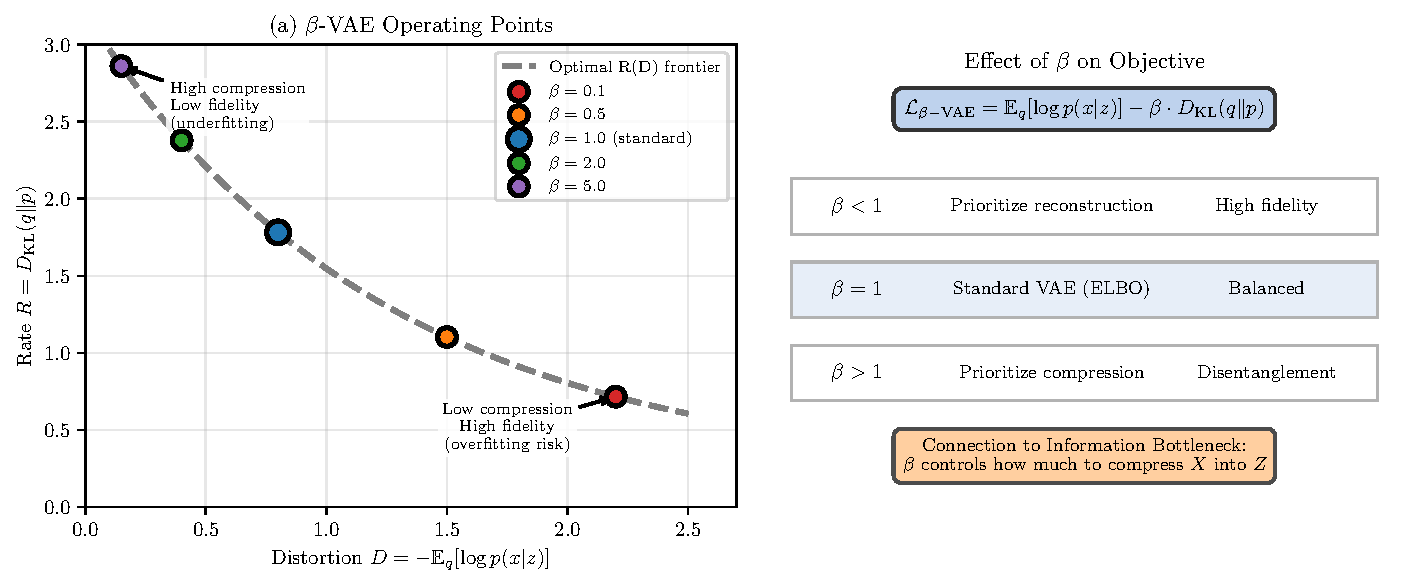
\includegraphics[width=\linewidth]{code/figures/ch08_variational_flows/fig_8_10_beta_vae.pdf}
\caption{$\beta$-VAE traces the rate--distortion frontier: higher $\beta$ enforces tighter alignment with the prior (lower rate) at the expense of reconstruction fidelity.}
\label{fig:beta_vae_tradeoff}
\end{figure}

\vspace{0.3cm}
\textbf{Prior choice.} Standard Gaussian priors keep KL analytic and work cleanly with bits-back; richer priors (VampPrior, autoregressive/flow priors) can reduce mismatch with the aggregated posterior at added complexity.
\section{Bits-Back Coding: Why the ELBO is Exactly Right}
\label{sec:bitsback}
%==========================

\vspace{1em}

\subsection{Compression as a Lens on Modeling}

In Chapter 1, we saw that minimizing cross-entropy is equivalent to minimizing codelength under an arithmetic coding scheme. A model that assigns high probability to the data compresses it well; a model that assigns low probability wastes bits. This connection between probability and compression runs deeper than it might first appear. It turns out that the ELBO is not just a convenient lower bound for training; it is the expected codelength achieved by a principled coding scheme called bits-back coding (up to small startup/shutdown overhead).

\vspace{0.3cm}

To understand this connection, imagine you want to transmit data $x$ to a receiver who shares your model $p_\theta(z)$ and $p_\theta(x \mid z)$. A naive approach would be to sample $z \sim p_\theta(z)$, send it using $-\log p_\theta(z)$ nats, then send $x$ conditioned on $z$ using $-\log p_\theta(x \mid z)$ nats. The total cost is $-\log p_\theta(z) - \log p_\theta(x \mid z)$ nats in expectation over $z$.

\vspace{0.3cm}

But this is wasteful. You had to sample $z$ anyway, which required generating randomness. That randomness is not arbitrary; it is structured by the distribution $p_\theta(z)$. Bits-back coding shows that you can reclaim some of that randomness by using the posterior $q_\phi(z \mid x)$ to "store" information, effectively getting back bits that would otherwise be wasted.

\vspace{1.5em}

\subsection{The Bits-Back Protocol: Step by Step}

Here is how bits-back coding works in detail. The sender and receiver share the model $(p_\theta(z), p_\theta(x \mid z))$ and the approximate posterior $q_\phi(z \mid x)$. They also share a reversible entropy coding scheme (or, equivalently, a stream of bits/state) that lets them sample from a distribution using bits and recover those bits during decoding.

\vspace{0.3cm}

\textbf{Encoding:}

1. The sender wants to transmit data point $x$.

2. The sender samples $z \sim q_\phi(z \mid x)$ using bits from the shared coder/state. This consumes $-\log q_\phi(z \mid x)$ nats of randomness on average.

3. The sender transmits $z$ using the prior $p_\theta(z)$ as a coding distribution. This costs $-\log p_\theta(z)$ nats.

4. The sender transmits $x$ using the likelihood $p_\theta(x \mid z)$ as a coding distribution. This costs $-\log p_\theta(x \mid z)$ nats.

5. Here is the key: the $-\log q_\phi(z \mid x)$ nats of randomness used to sample $z$ can be recycled. Because the coder is reversible, decoding $z$ under $q_\phi(z \mid x)$ returns those bits to the shared state. In the codelength bookkeeping, this appears as a $+\log q_\phi(z \mid x)$ credit.

\vspace{0.3cm}

\begin{figure}[t]
\centering
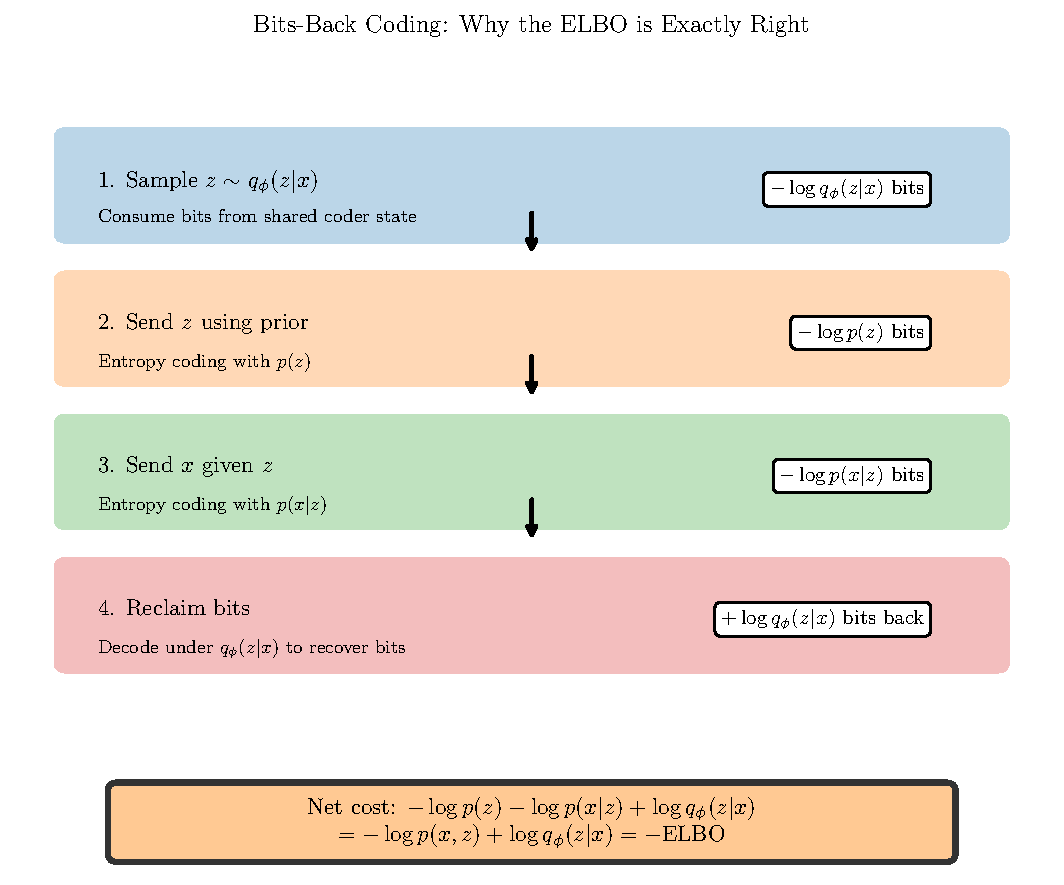
\includegraphics[width=\linewidth]{code/figures/ch08_variational_flows/fig_8_4_bitsback_protocol.pdf}
\caption{Bits-back coding reuses encoder randomness: sample from $q_\phi(z\mid x)$, transmit under the prior and likelihood, then reclaim the posterior bits to achieve codelength equal to $-\mathrm{ELBO}$.}
\label{fig:bitsback_protocol}
\end{figure}

\vspace{0.3cm}

The net codelength is:
%
\begin{equation}
-\log p_\theta(z) - \log p_\theta(x \mid z) + \log q_\phi(z \mid x)
= -\log p_\theta(x, z) + \log q_\phi(z \mid x)
\end{equation}

\vspace{0.3cm}

Taking the expectation over $z \sim q_\phi(z \mid x)$, we get:
%
\begin{equation}
\mathbb{E}_{q_\phi} [-\log p_\theta(x, z) + \log q_\phi(z \mid x)] = -\text{ELBO}(q_\phi, \theta; x)
\end{equation}

\vspace{0.3cm}

The expected codelength of this bits-back construction is $-\text{ELBO}(q_\phi,\theta;x)$, up to the startup/shutdown overhead discussed below. So maximizing the ELBO corresponds to minimizing expected codelength for the compressor induced by $(p_\theta, q_\phi)$.

\vspace{1.5em}

\begin{keyinsight}
Bits-back coding turns the ELBO from an abstract bound into a concrete compression algorithm. The reconstruction term $\mathbb{E}_{q_\phi}[\log p_\theta(x \mid z)]$ measures the cost of encoding $x$ given $z$. The KL term $D_{\text{KL}}(q_\phi \| p_\theta)$ measures the net cost of encoding $z$ after reclaiming bits from the posterior. Training a VAE by maximizing the ELBO is exactly training a compressor by minimizing expected codelength.
\end{keyinsight}

\vspace{1.5em}

\subsection{Why This Matters: Interpretation and Motivation}

The bits-back perspective gives us several valuable insights:

\vspace{0.3cm}

\textbf{The ELBO is not arbitrary.} For a given latent-variable model and approximate posterior, it is the objective that drops out of building an efficient bits-back compressor. Changing it either changes the coding scheme or wastes bits.

\vspace{0.3cm}

\textbf{The reconstruction-regularization tradeoff has a coding interpretation.} Better reconstruction means fewer bits to encode $x$ given $z$. Lower KL means fewer net bits to encode $z$ under the prior after accounting for bits back. The optimal posterior balances these two costs.

\vspace{0.3cm}

\textbf{Amortization makes sense.} Training an amortized encoder $q_\phi(z \mid x)$ across many examples is like designing a universal compressor that works well on average. The amortization gap is the difference between this universal compressor and the best compressor for a specific $x$.

\vspace{0.3cm}

\textbf{Tighter bounds mean better compression.} If we use a more flexible posterior family or importance-weighted objectives (like IWAE), we reduce the gap between the ELBO and the true log-evidence, which corresponds to improving compression efficiency.

\vspace{1.5em}

\begin{examplebox}
\textbf{Worked Example: Compressing MNIST Digits}

Suppose we train a VAE on MNIST digits with a 10-dimensional latent space. Each image is 784 pixels, each pixel in [0, 255]. Uncompressed, each image requires $784 \times 8 = 6272$ bits.

A trained VAE might achieve an ELBO of approximately $-100$ nats per image, which is $-100 / \log 2 \approx 144$ bits. \emph{Numbers are approximate and will vary with architecture, dataset preprocessing, optimization, and training budget.} This is a dramatic compression: from 6272 bits to 144 bits, a 43x reduction.

The breakdown is roughly:
- KL term: $\approx 10$ nats (encoding which point in the latent space)
- Reconstruction term: $\approx 90$ nats (encoding pixel values given latent code)

The bits-back interpretation says that we spend $-\log p_\theta(z) \approx 15$ nats sending $z$ under the prior, spend $\approx 90$ nats sending the image conditioned on $z$, and reclaim $\log q_\phi(z \mid x) \approx 5$ nats from the posterior randomness, for a net cost of $15 + 90 - 5 = 100$ nats.
\end{examplebox}

\vspace{2em}

%==========================

\vspace{0.3cm}
\begin{keyinsight}
\textbf{What rate does bits-back achieve?} If you encode $x$ by choosing $z\sim q_\phi(z\mid x)$ and then sending $z$ under $p_\theta(z)$ and $x$ under $p_\theta(x\mid z)$, you pay
$$\mathbb{E}_{q_\phi}[{-}\log p_\theta(z)] + \mathbb{E}_{q_\phi}[{-}\log p_\theta(x\mid z)].$$
Bits-back returns the entropy of $q_\phi(z\mid x)$ as usable bits. Using the identity
$$\mathbb{E}_{q_\phi}[{-}\log p_\theta(z)] = D_{\mathrm{KL}}(q_\phi\|p_\theta) + \mathbb{E}_{q_\phi}[{-}\log q_\phi(z\mid x)],$$
the last term is exactly what the decoder gets back. The net expected codelength is therefore
$$\mathbb{E}_{q_\phi}[{-}\log p_\theta(x\mid z)] + D_{\mathrm{KL}}(q_\phi\|p_\theta) \;=\; -\mathrm{ELBO},$$
up to the small startup/shutdown overhead below. The remaining gap to the optimal codelength under the model, $-\log p_\theta(x)$, is $D_{\mathrm{KL}}(q_\phi(z\mid x)\,\|\,p_\theta(z\mid x))$: bits-back makes the \emph{variational} code efficient, but it cannot beat a mismatched posterior.
\end{keyinsight}

\vspace{0.3cm}
\begin{keyinsight}
\textbf{Startup/shutdown overhead.} Streaming bits-back (e.g., with ANS) incurs $\mathcal{O}(D_{\mathrm{KL}}(q\|p))$ bits of state per sequence. Amortized over a length-$n$ stream this adds $\approx D_{\mathrm{KL}}(q\|p)/n$ nats per symbol, negligible when $n\gg 1$.
\end{keyinsight}

\section{Three Gaps: Approximation, Amortization, and Optimization}
\label{sec:three_gaps}
%==========================

\vspace{1em}

\subsection{Why VAEs Don't Reach Optimal Compression}

When we train a VAE, we are not directly optimizing log-likelihood. We are optimizing a lower bound that depends on our choice of approximate posterior family and our ability to find good parameters. This means there are several sources of suboptimality, which we can organize into three distinct gaps.

\vspace{0.3cm}

Understanding these gaps is crucial for diagnosing why a VAE might underperform and for choosing interventions to improve it. Each gap has different causes and requires different solutions.

\vspace{1.5em}

\begin{figure}[t]
\centering
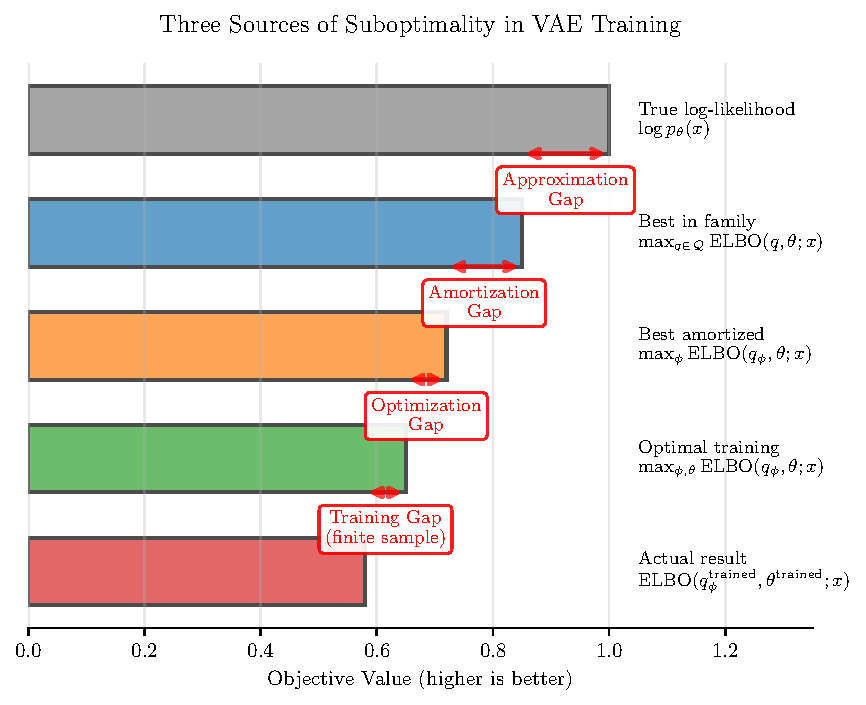
\includegraphics[width=\linewidth]{code/figures/ch08_variational_flows/fig_8_5_three_gaps.pdf}
\caption{Three sources of ELBO slack: approximation (posterior family limits), amortization (encoder sharing), and optimization (training quality). Diagnose which gap dominates before choosing interventions.}
\label{fig:three_gaps}
\end{figure}

\vspace{1.5em}

\subsection{The Approximation Gap}

The approximation gap is the difference between the true posterior $p_\theta(z \mid x)$ and the best approximation we could achieve within our chosen family $\mathcal{Q}$. Formally:
%
\begin{equation}
\text{Approximation Gap} = D_{\text{KL}}(q^*(z \mid x) \| p_\theta(z \mid x))
\end{equation}
%
where $q^*(z \mid x) = \arg\min_{q \in \mathcal{Q}} D_{\text{KL}}(q(z \mid x) \| p_\theta(z \mid x))$.

\vspace{0.3cm}

This gap arises from limitations of the family $\mathcal{Q}$. If we choose $\mathcal{Q}$ to be all diagonal Gaussian distributions but the true posterior is multimodal, no member of $\mathcal{Q}$ can match the true posterior well. The family is simply not expressive enough.

\vspace{0.3cm}

Common sources of approximation gaps include:

\vspace{0.3cm}

\textbf{Mean-field assumptions.} Assuming $q(z \mid x) = \prod_j q(z_j \mid x)$ (factorized across dimensions) when the true posterior has strong correlations. This is fast to compute but misses dependencies.

\vspace{0.3cm}

\textbf{Uni-modal distributions.} Using a Gaussian $q(z \mid x)$ when the true posterior has multiple modes. The Gaussian will average over modes, missing the multimodal structure.

\vspace{0.3cm}

\textbf{Fixed-form families.} Using a specific parametric form (Gaussian, Laplace, etc.) when the true posterior has heavier tails or different shape.

\vspace{0.3cm}

To reduce the approximation gap, we can use more flexible families: normalizing flows applied to the posterior (flow-based VAEs), mixture distributions, or implicit distributions parameterized by neural samplers.

\vspace{1.5em}

\subsection{The Amortization Gap}

The amortization gap is the difference between the best family member $q^*(z \mid x)$ and what the amortized encoder actually produces $q_\phi(z \mid x)$:
%
\begin{equation}
\text{Amortization Gap} = D_{\text{KL}}(q_\phi(z \mid x) \| q^*(z \mid x))
\end{equation}

\vspace{0.3cm}

The word "amortized" means we use a single set of parameters $\phi$ to encode all examples, rather than optimizing separate parameters for each $x$. This is essential for scalability---we cannot afford to run full variational inference for every data point. But it means the encoder must compress all the variation across the dataset into a fixed network architecture.

\vspace{0.3cm}

For some examples, the encoder might do very well. For others, it might produce a poor posterior approximation even though a better one exists in the family $\mathcal{Q}$. The amortization gap captures this shortfall.

\vspace{0.3cm}

Common causes of amortization gaps include:

\vspace{0.3cm}

\textbf{Encoder capacity.} The encoder network might not be expressive enough to capture the complexity of the mapping from $x$ to posterior parameters.

\vspace{0.3cm}

\textbf{Out-of-distribution examples.} Examples that are rare in the training set might get poor posterior approximations because the encoder never learned to handle them well.

\vspace{0.3cm}

\textbf{Local optima.} The encoder might get stuck in poor solutions for some inputs due to optimization difficulties.

\vspace{0.3cm}

To measure the amortization gap, we can compare the amortized ELBO to a refined ELBO where we do additional optimization of $\phi$ for each specific $x$ (holding $\theta$ fixed). The difference reveals how much the amortization is costing us.


\vspace{0.5em}

\subsection{The Optimization Gap}

The optimization gap is the difference between what we actually achieve during training and what we could achieve if optimization were perfect:
%
\begin{equation}
\text{Optimization Gap} = \text{ELBO}(q^*_\phi, \theta^*; x) - \text{ELBO}(q_\phi, \theta; x)
\end{equation}
%
where $(q^*_\phi, \theta^*)$ are the optimal parameters for the ELBO objective.

\vspace{0.3cm}

This gap arises from practical limitations of stochastic gradient descent: finite training time, learning rate schedules, local optima, gradient noise from minibatch sampling, and all the other challenges of neural network training.

\vspace{0.3cm}

Unlike the approximation and amortization gaps, which are structural limitations of the model, the optimization gap is a training artifact. With better optimization or more compute, we could reduce it. In practice, standard techniques from deep learning (learning rate schedules, gradient clipping, architecture search, regularization) address this gap.

\vspace{1.5em}

\begin{pausebox}
\textbf{Pause and Diagnose.} If your VAE is performing poorly, which gap is the likely culprit? Check the reconstruction quality on training examples. If it is poor even for well-seen examples, you likely have an optimization or amortization gap. If reconstructions are good but generations are poor, you may have an approximation gap (the posterior family cannot match the true posterior, leading to a mismatch between encoding and generation). If held-out likelihood is much worse than training likelihood, the optimization or amortization gap is probably large.
\end{pausebox}

\vspace{2em}

%==========================
\section{Normalizing Flows: Exact Likelihoods Through Invertible Maps}
\label{sec:flows}
%==========================

\vspace{1em}

\subsection{The Limits of Variational Bounds}

VAEs give us flexible latent variable models, but they come with a fundamental limitation: we optimize a lower bound on log-likelihood, not the likelihood itself. The gap between the ELBO and the true log-evidence is the KL divergence between our approximate posterior and the true posterior. This gap is exactly zero only when $q_\phi(z\mid x)=p_\theta(z\mid x)$ (i.e., when the true posterior lies in our chosen family and we find it).

\vspace{0.3cm}

Normalizing flows take a different approach. Instead of introducing latent variables and approximating their posterior, they directly transform a simple base distribution (like a standard Gaussian) into the data distribution using an invertible map. Because the map is invertible, we can compute exact likelihoods using the change-of-variables formula, with no variational approximation required.

\vspace{0.3cm}

The tradeoff is complexity. Flows require carefully designed architectures to ensure invertibility and efficient Jacobian computation. They do not provide a compressed latent representation in the same way VAEs do. But when exact likelihood is crucial---for density estimation, anomaly detection, or lossless compression---flows can be the right choice.

\vspace{1.5em}

\subsection{The Change-of-Variables Formula}

Suppose we have a simple base distribution $p_0(z)$ (typically $\mathcal{N}(0, I)$) and an invertible, differentiable map $f: \mathbb{R}^d \to \mathbb{R}^d$. If we transform samples $z \sim p_0(z)$ through $f$ to get $x = f(z)$, what is the distribution of $x$?

\vspace{0.3cm}

The answer comes from the change-of-variables formula. For invertible $f$, the density of $x$ is:
%
\begin{equation}
p(x) = p_0(f^{-1}(x)) \left| \det \frac{\partial f^{-1}}{\partial x} \right|
\end{equation}

\vspace{0.3cm}

Taking logs:
%
\begin{equation}
\log p(x) = \log p_0(f^{-1}(x)) + \log \left| \det J_{f^{-1}}(x) \right|
\end{equation}
%
where $J_{f^{-1}}(x) = \frac{\partial f^{-1}}{\partial x}$ is the Jacobian matrix of the inverse map.

\vspace{0.3cm}

Equivalently, writing $z=f^{-1}(x)$ and using $J_{f^{-1}}(x)=J_f(z)^{-1}$, we can rewrite this as
%
\begin{equation}
\log p(x)=\log p_0(z) - \log|\det J_f(z)|.
\end{equation}
%
We will use whichever form makes the Jacobian computation easiest.

\vspace{0.3cm}

This formula has two terms. The first term, $\log p_0(f^{-1}(x))$, measures how probable the corresponding base point $z = f^{-1}(x)$ is under the simple distribution. The second term, $\log |\det J_{f^{-1}}(x)|$, is a correction factor that accounts for how the map $f$ distorts volume.

\vspace{0.3cm}

If $f$ locally compresses space (the Jacobian determinant is less than 1), we add a positive correction to the log-density because the same amount of probability mass is now squeezed into a smaller volume. If $f$ locally expands space (determinant greater than 1), we subtract from the log-density because the probability mass is spread out.

\vspace{1.5em}

\begin{geometrylens}
The change-of-variables formula is fundamentally geometric. Density is probability mass per unit volume. When we transform space, we change volumes. The Jacobian determinant measures exactly how volumes scale under the transformation. A region that was volume $V$ in $z$-space becomes volume $|\det J_f| \cdot V$ in $x$-space. To preserve total probability mass, density must scale inversely: if volume increases by a factor $\alpha$, density decreases by $1/\alpha$.
\end{geometrylens}

\vspace{1.5em}

\begin{figure}[t]
\centering
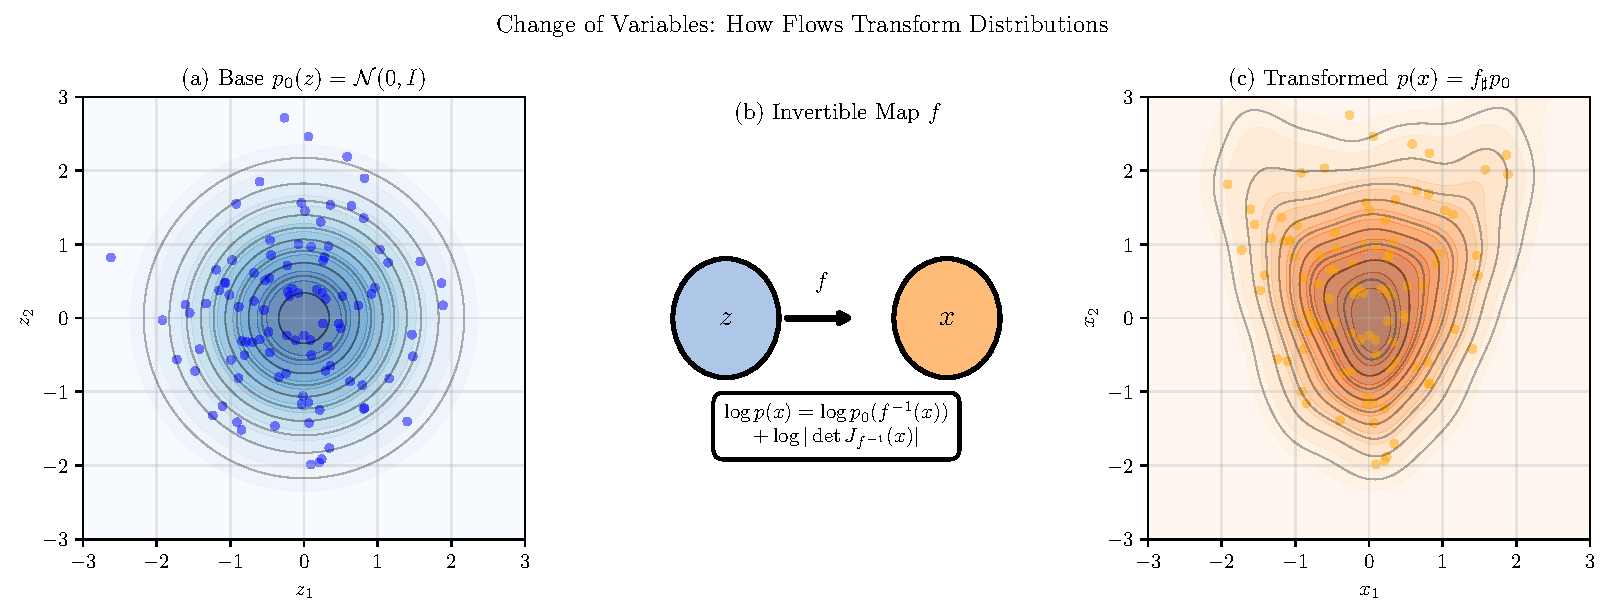
\includegraphics[width=\linewidth]{code/figures/ch08_variational_flows/fig_8_7_change_of_variables.pdf}
\caption{Change of variables decomposes $\log p(x)$ into the base log-density and a Jacobian term capturing local volume expansion or contraction under the invertible map.}
\label{fig:change_of_variables}
\end{figure}

\vspace{1.5em}

\subsection{The Computational Challenge: Efficient Jacobians}

The change-of-variables formula looks simple, but there is a hidden cost: computing $\det J_{f^{-1}}(x)$ for a general function $f: \mathbb{R}^d \to \mathbb{R}^d$ requires $O(d^3)$ operations (matrix determinant), and computing the Jacobian itself requires $O(d^2)$ operations. For high-dimensional data like images (where $d$ might be tens of thousands), this is prohibitively expensive.

\vspace{0.3cm}

The key to practical flows is restricting $f$ to architectures where the Jacobian has special structure that makes the determinant cheap to compute. There are three main design patterns:

\vspace{1.5em}

\subsection{Coupling Layers: RealNVP and Beyond}

A coupling layer splits the input into two parts, $(x_a, x_b)$, transforms only one part as a function of the other, and leaves the other part unchanged. The simplest version keeps $x_a$ fixed and transforms $x_b$:
%
\begin{align}
z_a &= x_a \\
z_b &= x_b \odot \exp(s(x_a)) + t(x_a)
\end{align}
%
where $s$ and $t$ are arbitrary neural networks (the scale and translation functions), and $\odot$ denotes element-wise multiplication.

\vspace{0.3cm}

The Jacobian of this transformation is:
%
\begin{equation}
J_f = \begin{pmatrix}
I & 0 \\
\frac{\partial z_b}{\partial x_a} & \text{diag}(\exp(s(x_a)))
\end{pmatrix}
\end{equation}

\vspace{0.3cm}

This Jacobian is block triangular; crucially, the bottom-right block $\frac{\partial z_b}{\partial x_b}$ is \emph{diagonal} (for affine couplings), so the determinant reduces to the product of those diagonal entries:
%
\begin{equation}
\log |\det J_f| = \sum_j s_j(x_a)
\end{equation}
%
where $s_j$ are the components of $s(x_a)$.

\vspace{0.3cm}

The computation is $O(d)$ instead of $O(d^3)$, making it tractable even for very high dimensions. The inverse is also easy to compute:
%
\begin{align}
x_a &= z_a \\
x_b &= (z_b - t(z_a)) \odot \exp(-s(z_a))
\end{align}

\begin{figure}[t]
\centering
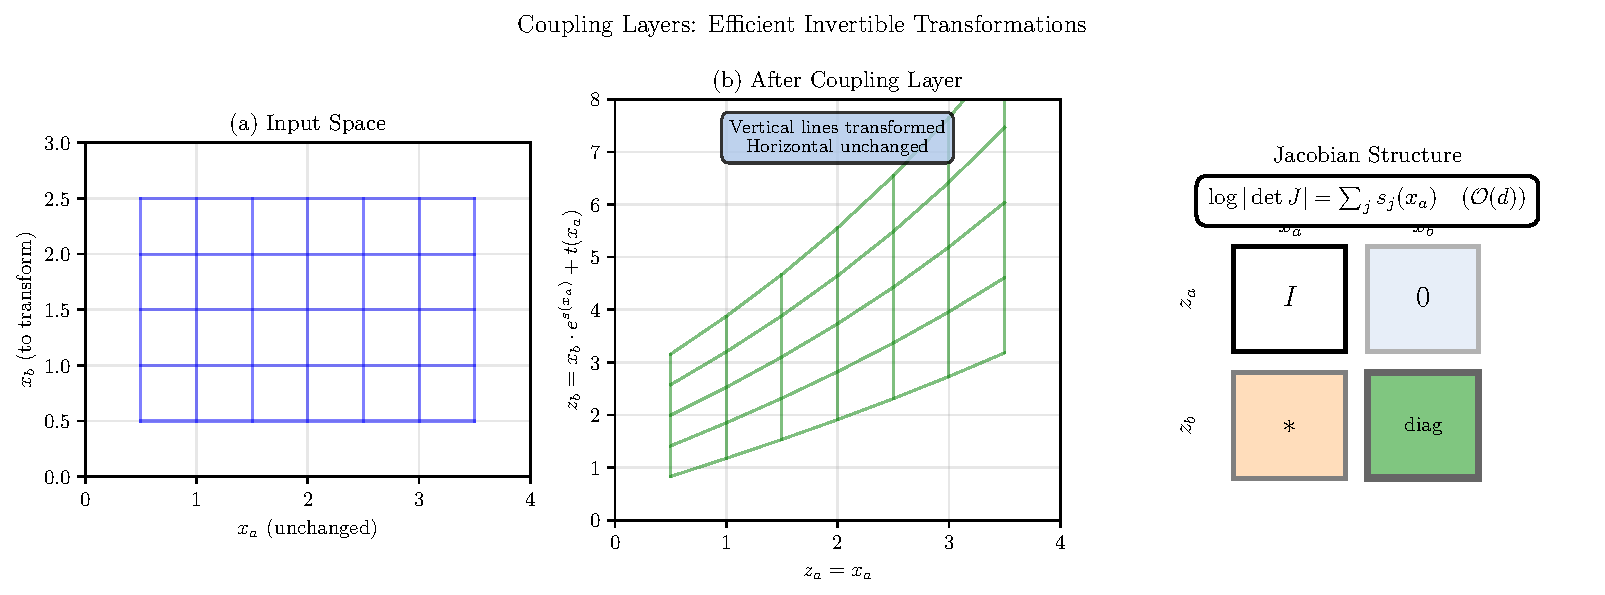
\includegraphics[width=\linewidth]{code/figures/ch08_variational_flows/fig_8_6_coupling_layer.pdf}
\caption{RealNVP-style coupling layers keep part of the vector fixed while scaling and shifting the remainder, yielding a block-triangular Jacobian with a cheap log-determinant.}
\label{fig:coupling-geometry}
\end{figure}

\vspace{0.5em}


\vspace{0.3cm}

By stacking multiple coupling layers with different partitions of dimensions (alternating which half is transformed), we build an expressive invertible map.

\vspace{1.5em}

\begin{examplebox}
\textbf{Worked Example: 2D Coupling Layer}

Let $x = (x_1, x_2) \in \mathbb{R}^2$. A coupling layer might use $x_a = x_1$ and $x_b = x_2$:
%
\begin{align*}
z_1 &= x_1 \\
z_2 &= x_2 \cdot \exp(s(x_1)) + t(x_1)
\end{align*}

Suppose $s(x_1) = 0.5 x_1$ and $t(x_1) = x_1^2$. For input $x = (2, 3)$:
%
\begin{align*}
z_1 &= 2 \\
z_2 &= 3 \cdot \exp(1) + 4 \approx 12.15
\end{align*}

The log-determinant is:
%
\begin{equation*}
\log |\det J_f| = s(x_1) = 0.5 \cdot 2 = 1
\end{equation*}

To invert: given $z = (2, 12.15)$, we compute:
%
\begin{align*}
x_1 &= 2 \\
x_2 &= (12.15 - 4) / \exp(1) \approx 3
\end{align*}

The coupling structure makes both forward and inverse efficient.
\end{examplebox}

\vspace{1.5em}

\subsection{Autoregressive Flows: MAF and IAF}

Autoregressive flows impose a causal ordering on dimensions: $x_i$ depends only on $x_1, \ldots, x_{i-1}$. The transformation is:
%
\begin{equation}
z_i = \frac{x_i - \mu_i(x_{<i})}{\sigma_i(x_{<i})}
\end{equation}
%
where $\mu_i$ and $\sigma_i$ are functions of previous dimensions.

\vspace{0.3cm}

The Jacobian is block-triangular (identity on the frozen block, triangular on the transformed block) by construction, so the determinant is again the product of diagonal entries:
%
\begin{equation}
\log |\det J_f| = -\sum_i \log \sigma_i(x_{<i})
\end{equation}

\vspace{0.3cm}

There are two variants depending on the direction of dependency:

\vspace{0.3cm}

\textbf{Masked Autoregressive Flow (MAF).} We parameterize $z$ as an autoregressive function of $x$. Given $x$, we can compute all $\mu_i(x_{<i})$ and $\sigma_i(x_{<i})$ in one masked forward pass, so evaluating $\log p(x)$ is fast. But sampling is slow because generating $x$ from $z$ requires sequential inversion.

\vspace{0.3cm}

\textbf{Inverse Autoregressive Flow (IAF).} We parameterize $x$ as an autoregressive function of $z$. Now sampling is fast (one masked forward pass computes all $x_i$), but evaluating $\log p(x)$ is slow because it requires sequential inversion. This makes IAF fast for generation, slow for density evaluation.

\vspace{0.3cm}

The choice between MAF and IAF depends on whether you care more about evaluating densities (MAF) or generating samples (IAF). For tasks like density estimation or anomaly detection, use MAF. For generative modeling where you mostly sample, use IAF.

\vspace{1.5em}

\subsection{Continuous Normalizing Flows: Neural ODEs}

Instead of composing discrete layers, continuous normalizing flows define a continuous-time evolution:
%
\begin{equation}
\frac{dx}{dt} = v_\theta(x, t)
\end{equation}
%
where $v_\theta$ is a neural network defining a velocity field.

\vspace{0.3cm}

Starting from $x(0) = z \sim p_0(z)$, we integrate this ODE to time $T$ to get $x(T) = f(z)$, where $f$ is now defined implicitly by the ODE solution rather than explicitly as a composition of layers.

\vspace{0.3cm}

The change-of-variables formula becomes an integral. The log-density evolves according to:
%
\begin{equation}
\frac{d \log p(x(t))}{dt} = -\text{tr}\left( \frac{\partial v_\theta}{\partial x} \right)
\end{equation}

\vspace{0.3cm}

Integrating from $0$ to $T$:
%
\begin{equation}
\log p(x(T)) = \log p_0(x(0)) - \int_0^T \text{tr}\left( \frac{\partial v_\theta}{\partial x(t)} \right) dt
\end{equation}

\vspace{0.3cm}

The trace of the Jacobian appears instead of the determinant because we are dealing with infinitesimal transformations. For a small step $dt$, the map is approximately $x + v_\theta(x,t) dt$, with Jacobian $I + \frac{\partial v_\theta}{\partial x} dt$. The log-determinant is $\log \det(I + A dt) \approx \text{tr}(A) dt$ for small $dt$.

\vspace{0.3cm}

Computing the trace exactly is still expensive ($O(d)$ for each entry, times $d$ entries = $O(d^2)$), but the Hutchinson trace estimator allows unbiased stochastic estimation with just $O(d)$ cost per sample using random vectors.

\vspace{0.3cm}

Continuous flows offer several advantages: they can be more parameter-efficient than stacking discrete layers, they naturally handle irregularly-sampled time series, and they provide a smooth interpolation between base and data distributions. The cost is more expensive training due to ODE solving and trace estimation.

\vspace{2em}

%==========================
\section{VAEs vs Flows: Complementary Strengths}
\label{sec:vae_vs_flows}
%==========================

\vspace{1em}

\begin{figure}[t]
\centering
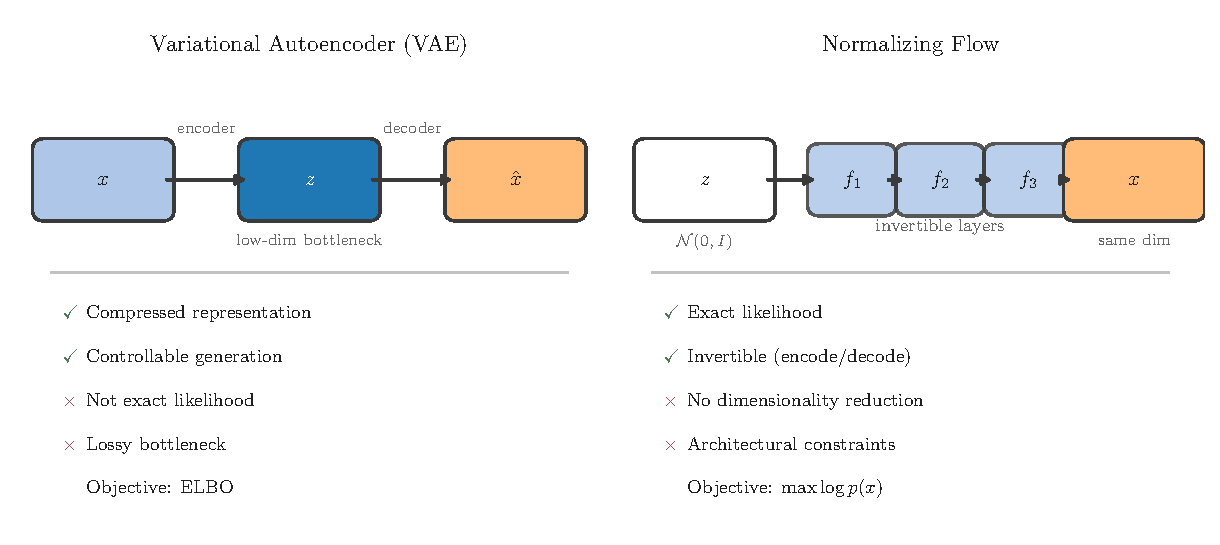
\includegraphics[width=\linewidth]{code/figures/ch08_variational_flows/fig_8_8_vae_vs_flow.pdf}
\caption{VAEs compress through a low-dimensional bottleneck and optimize the ELBO; flows preserve dimensionality, offer exact likelihoods, and rely on invertible maps.}
\label{fig:vae_vs_flow}
\end{figure}

\vspace{1em}

\subsection{What VAEs Offer}

Variational autoencoders excel at learning compressed, meaningful latent representations. The bottleneck through a low-dimensional $z$ forces the encoder to extract essential features while discarding noise and irrelevant details. This makes VAEs particularly valuable for:

\vspace{0.3cm}

\textbf{Controllable generation.} By learning a structured latent space, we can manipulate specific attributes by moving through $z$-space. Want to change the smile in a face? Move along the discovered "smile direction."

\vspace{0.3cm}

\textbf{Semi-supervised learning.} The learned representations $q_\phi(z \mid x)$ often transfer well to downstream tasks, providing useful features for classification or regression with limited labels.

\vspace{0.3cm}

\textbf{Lossy compression.} For applications where perfect reconstruction is not needed, VAEs provide a principled way to compress data through a low-dimensional code.

\vspace{0.3cm}

\textbf{Interpretability.} Low-dimensional latent spaces can be visualized and understood, revealing structure in the data.

\vspace{0.3cm}

The downside is the variational gap: VAEs optimize a lower bound, not exact likelihood, and the learned representations may not fully capture all information in the data.

\vspace{1.5em}

\subsection{What Flows Offer}

Normalizing flows excel at exact density modeling without lossy compression. They provide:

\vspace{0.3cm}

\textbf{Exact likelihoods.} No variational gap, no lower bounds. The likelihood you compute is the true likelihood under your model.

\vspace{0.3cm}

\textbf{Invertibility.} You can move freely between data space and latent space, encoding and decoding without information loss.

\vspace{0.3cm}

\textbf{Lossless compression.} Exact likelihoods let you pair a flow with an entropy coder for lossless compression. If the flow fits the data distribution well, the resulting rates can be near-optimal.

\vspace{0.3cm}

\textbf{Precise anomaly detection.} Exact densities allow confident identification of out-of-distribution samples based on likelihood thresholds.

\vspace{0.3cm}

The downsides are computational cost (especially for high-dimensional data), architectural constraints (ensuring invertibility and efficient Jacobians), and lack of dimensionality reduction (the latent space has the same dimension as data space).

\vspace{1.5em}

\subsection{Hybrid Approaches: Best of Both Worlds}

Many modern architectures combine VAEs and flows to use both strengths:

\vspace{0.3cm}

\textbf{Flow-based posteriors.} Use a normalizing flow to model the approximate posterior $q_\phi(z \mid x)$ in a VAE, increasing flexibility while maintaining tractable ELBO computation.

\vspace{0.3cm}

\textbf{Flow priors.} Replace the simple Gaussian prior $p_\theta(z)$ in a VAE with a flow-based prior, allowing more expressive latent distributions.

\vspace{0.3cm}

\textbf{Flow decoders.} Use a flow as the decoder $p_\theta(x \mid z)$, getting exact likelihoods for the reconstruction term in the ELBO.

\vspace{0.3cm}

\textbf{Latent flows.} Apply flows in the low-dimensional latent space of a VAE rather than in high-dimensional data space, reducing computational cost while gaining expressivity.

\vspace{0.3cm}

These hybrids illustrate a broader principle: different components of a generative model can use different techniques depending on their role. There is no single "best" architecture, only architectures better suited to specific tasks and constraints.

\vspace{2em}

%==========================
\section{Posterior Collapse and the Latent Bottleneck}
\label{sec:posterior_collapse}
%==========================

\vspace{1em}

\subsection{When the Decoder is Too Strong}

One of the most frustrating phenomena in VAE training is posterior collapse: the model learns to ignore the latent variable $z$ entirely. The approximate posterior $q_\phi(z \mid x)$ becomes indistinguishable from the prior $p_\theta(z)$ for all $x$, making the KL term in the ELBO vanish. Meanwhile, the decoder $p_\theta(x \mid z)$ learns to generate $x$ without actually using $z$.

\vspace{0.3cm}

Why does this happen? The ELBO objective has two terms that push in opposite directions. The reconstruction term encourages using $z$ to improve predictions. The KL term encourages making the posterior close to the prior, which means making it less informative about $x$. When the decoder is expressive enough to model $x$ well on its own (for example, an autoregressive decoder in a sequence VAE), the easiest way to maximize the ELBO is to simply ignore $z$ and let the decoder do all the work.

\vspace{0.3cm}

Mathematically, if $p_\theta(x \mid z) \approx p_\theta(x)$ (the decoder does not actually depend on $z$), then the optimal posterior is $q_\phi(z \mid x) = p_\theta(z)$ regardless of $x$. This makes the KL term zero, and the reconstruction term becomes just the marginal log-likelihood $\log p_\theta(x)$. The model has degenerated into a decoder-only model with no meaningful latent structure.

\vspace{1.5em}

\begin{figure}[t]
\centering
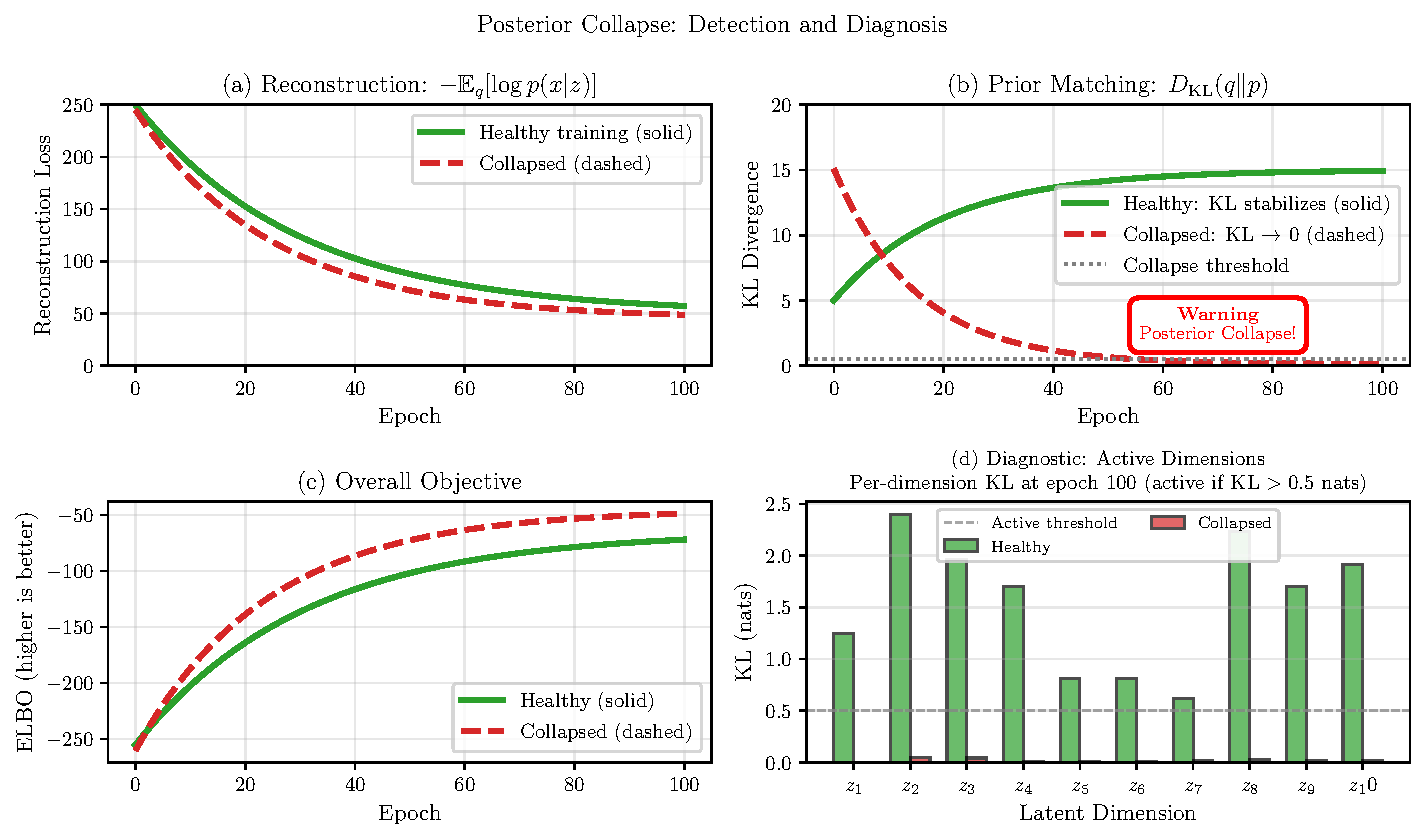
\includegraphics[width=\linewidth]{code/figures/ch08_variational_flows/fig_8_9_posterior_collapse.pdf}
\caption{Posterior collapse: the encoder's outputs shrink toward the prior, KL drops to zero, and the decoder learns to ignore $z$, defeating the latent bottleneck.}
\label{fig:posterior_collapse}
\end{figure}

\vspace{1.5em}

\subsection{Why This is Bad}

Posterior collapse defeats the purpose of using a latent variable model. We wanted $z$ to capture meaningful structure, enable manipulation of generated samples, provide compressed representations, or support semi-supervised learning. If $z$ is ignored, we get none of these benefits.

\vspace{0.3cm}

Moreover, the collapsed model is often worse at generation than it should be. Without using $z$, the decoder must fit the entire data distribution directly, which can be harder than factoring the problem into "encode to $z$, decode from $z$."

\vspace{0.3cm}

Posterior collapse is especially common in sequence VAEs for text. Autoregressive decoders (like LSTMs or transformers) are so expressive that they can generate coherent text without any latent variable. The VAE objective provides no incentive to use $z$ if the decoder can achieve good reconstruction without it.

\vspace{1.5em}

\subsection{Preventing Collapse: Architectural and Objective Interventions}

Several techniques can prevent or mitigate posterior collapse:

\vspace{0.3cm}

\textbf{KL annealing.} Start training with a small weight on the KL term, gradually increasing it over time. This gives the encoder and decoder time to learn to use $z$ before the KL penalty becomes strong enough to push toward collapse. The schedule might look like:
%
\begin{equation}
\text{ELBO}_\beta = \mathbb{E}_{q_\phi}[\log p_\theta(x \mid z)] - \beta(t) \cdot D_{\text{KL}}(q_\phi \| p_\theta)
\end{equation}
%
where $\beta(t)$ increases from 0 to 1 over training.

\vspace{0.3cm}

\textbf{Free bits.} Prevent the KL term from dropping below a threshold per latent dimension, ensuring at least some information is encoded:
%
\begin{equation}
\text{ELBO}_{free} = \mathbb{E}_{q_\phi}[\log p_\theta(x \mid z)] - \sum_j \max(\lambda, D_{\text{KL}}(q_{\phi,j} \| p_{\theta,j}))
\end{equation}
%
where $\lambda$ is the free bits threshold (e.g., 0.5 nats per dimension).

\vspace{0.3cm}

\textbf{Weakening the decoder.} Make the decoder less expressive so it must rely on $z$. This might mean using a smaller network, removing some layers, or adding bottlenecks. The downside is potentially worse reconstruction.

\vspace{0.3cm}

\textbf{Auxiliary losses.} Add explicit objectives that encourage using $z$, such as predicting data attributes from $z$ or enforcing that nearby points in data space map to nearby points in latent space.

\vspace{0.3cm}

\textbf{Architecture design.} In sequence models, injecting $z$ at every decoder step (rather than just at initialization) can help ensure it is used. Conditioning on $z$ through attention mechanisms or gating can also increase utilization.

\vspace{1.5em}

\begin{pausebox}
\textbf{Pause and Experiment.} If you are training a VAE and suspect posterior collapse, check the KL term during training. If it drops to near zero and stays there, you have collapse. Try KL annealing or free bits. Also visualize latent codes: do different $x$ map to meaningfully different $z$? If all $z$ look the same regardless of $x$, the encoder is not learning anything useful.
\end{pausebox}

\vspace{2em}

%==========================

\vspace{0.3cm}
\textbf{Mechanics.} A strong decoder can fit $p_\theta(x\mid z)\approx p_\theta(x)$, ignoring $z$. Then $\nabla_\phi\,\mathbb{E}_{q_\phi}[\log p_\theta(x\mid z)]\approx 0$ while the KL still penalizes $I_q(x;z)$, pushing $q_\phi(z\mid x)\to p(z)$ unless we intervene.
\vspace{0.3cm}
\begin{examplebox}
\textbf{Toy collapse.} Train a text VAE (Transformer decoder) on a small corpus. With $\beta{=}1$ and no KL scheduling, KL $\to 0$ while recon stays high ($q(z\mid x)\approx p(z)$). Cyclical KL or lagging inference restores non-zero KL and $I_q(x;z)>0$.
\end{examplebox}
\section{Calibration: Beyond Likelihood}
\vspace{0.3cm}
\label{sec:calibration}
%==========================

\vspace{1em}

\subsection{Why Likelihood is Not Enough}

We have focused heavily on likelihood: the ELBO bounds it, bits-back coding compresses according to it, flows compute it exactly. But likelihood alone does not guarantee a good model. A model can assign high likelihood to data while making poor predictions about uncertainty, generating unrealistic samples, or failing to capture key statistical properties.

\vspace{0.3cm}

Calibration asks a different question: do the model's probabilistic predictions match reality? If the model says an event has 70% probability, does it actually happen 70% of the time? For a VAE or flow, this means checking not just that $p_\theta(x)$ is high for observed $x$, but that the model's uncertainties, reconstructions, and generations behave as expected.

\vspace{1.5em}

\subsection{Posterior Predictive Checks}

A useful diagnostic tool from Bayesian statistics is the posterior predictive check. The idea is to simulate data from the model and compare its statistical properties to real data. For a VAE, this means:

\vspace{0.3cm}

1. Take a data point $x$ from your test set

2. Encode it: sample $z \sim q_\phi(z \mid x)$

3. Decode it: sample $x' \sim p_\theta(x' \mid z)$

4. Check if $x'$ has similar statistics to $x$ and other real data

\vspace{0.3cm}

The "statistics" can be anything relevant to your domain: pixel intensity histograms for images, word frequency distributions for text, spatial correlations, edge densities, whatever captures the structure you care about.

\vspace{0.3cm}

If the model is well-calibrated, simulated $x'$ should be indistinguishable from real $x$ in terms of these statistics. If $x'$ systematically differs (for example, blurrier images, less diverse text, missing rare features), the model is poorly calibrated even if it has high likelihood.

\vspace{1.5em}

\subsection{Uncertainty Calibration}

For the approximate posterior $q_\phi(z \mid x)$, we can check calibration of uncertainty estimates. If $q_\phi$ gives high variance around some latent dimension, that dimension should actually be uncertain: different plausible $z$ values should lead to meaningfully different reconstructions.

\vspace{0.3cm}

One way to test this is to sample multiple $z$ from $q_\phi(z \mid x)$, decode each one, and measure the diversity of reconstructions. High posterior variance should correspond to high reconstruction diversity. If the posterior variance is high but reconstructions are nearly identical, the uncertainty is miscalibrated.

\vspace{0.3cm}

Similarly, for the reconstruction distribution $p_\theta(x \mid z)$, we can check if predicted variances match actual errors. If the model predicts high variance for some pixel but always reconstructs it accurately, the uncertainty is overestimated. If it predicts low variance but makes large errors, the uncertainty is underestimated.

\vspace{1.5em}

\subsection{Out-of-Distribution Detection}

One practical application of calibration is detecting out-of-distribution (OOD) examples: data that comes from a different distribution than the training set. Ideally, the model should assign low likelihood to OOD examples, but this often fails in practice.

\vspace{0.3cm}

For example, VAEs sometimes assign higher likelihood to certain OOD images than to in-distribution images, because the OOD images happen to lie in high-density regions of the learned distribution for the wrong reasons (they may be very smooth or have other features that the VAE learned to favor).

\vspace{0.3cm}

Better OOD detection can be achieved by looking at the latent representation: does $q_\phi(z \mid x)$ put mass in regions of latent space that were common during training? Or does it produce a $z$ that is far from any training latent code? The latter is a red flag for OOD data.

\vspace{0.3cm}

Flows can use exact likelihood for OOD detection, but they suffer from the same issues: likelihood is not always well-calibrated for distinguishing in-distribution from OOD. Hybrid methods that combine likelihood with latent space structure often work better.

\vspace{2em}

%==========================
\section{Bridging to Language Modeling}
\label{sec:language_modeling_bridge}
%==========================

\vspace{1em}

\subsection{Sequence VAEs: Latent Variables for Text}

In Chapter 1, we explored autoregressive language models that predict tokens sequentially without any latent variables. Sequence VAEs add a latent $z$ that encodes global information about the entire sequence, while the decoder still autoregressively generates tokens conditioned on $z$.

\vspace{0.3cm}

The model structure is:
- Prior: $p_\theta(z) = \mathcal{N}(0, I)$
- Decoder: $p_\theta(x_{1:T} \mid z) = \prod_{t=1}^T p_\theta(x_t \mid x_{<t}, z)$
- Encoder: $q_\phi(z \mid x_{1:T})$ (often using a BiLSTM or transformer to encode the full sequence)

\vspace{0.3cm}

The ELBO becomes:
%
\begin{equation}
\text{ELBO} = \mathbb{E}_{q_\phi} \left[ \sum_{t=1}^T \log p_\theta(x_t \mid x_{<t}, z) \right] - D_{\text{KL}}(q_\phi(z \mid x_{1:T}) \| p(z))
\end{equation}

\vspace{0.3cm}

This looks like the cross-entropy loss from Chapter 1, but with two additions: the expectation over latent codes $z$, and the KL regularization term.

\vspace{1.5em}

\subsection{What Does the Latent Capture?}

When sequence VAEs work well (avoiding posterior collapse), the latent $z$ captures high-level semantic information: topic, sentiment, writing style, discourse structure. The decoder then fills in the token-level details conditioned on this global context.

\vspace{0.3cm}

For example, in a VAE trained on news articles, $z$ might encode the topic (politics, sports, technology) and overall sentiment (positive, negative, neutral), while the decoder generates specific sentences and word choices consistent with that topic and sentiment.

\vspace{0.3cm}

This factorization can improve generation by providing more coherent global structure. Purely autoregressive models sometimes generate locally fluent text that drifts off-topic or becomes internally inconsistent. A latent variable that commits to a global plan can prevent such drift.

\vspace{1.5em}

\subsection{The Bits-Back View of Sequence Compression}

From the bits-back perspective, the ELBO measures codelength for sequences just as it does for images. The KL term pays bits to transmit which latent code we are using. The reconstruction term pays bits to transmit the specific tokens given that latent code.

\vspace{0.3cm}

If $z$ is well-chosen, it should reduce the conditional entropy of tokens: $H(x_t \mid x_{<t}, z) < H(x_t \mid x_{<t})$. This means that knowing $z$ makes the next token more predictable, reducing the per-token codelength.

\vspace{0.3cm}

The total codelength is:
%
\begin{equation}
-\text{ELBO} = D_{\text{KL}}(q_\phi \| p) + \mathbb{E}_{q_\phi} \left[ -\sum_t \log p_\theta(x_t \mid x_{<t}, z) \right]
\end{equation}

\vspace{0.3cm}

For effective compression, we need $z$ to capture predictive information that reduces the second term more than it costs in the first term. If $z$ is uninformative, we pay KL bits for nothing.

\vspace{1.5em}

\subsection{Amortization in Sequence Models}

The amortization gap is particularly relevant for sequence VAEs. The encoder $q_\phi(z \mid x_{1:T})$ must compress an entire sequence (potentially hundreds of tokens) into a low-dimensional $z$. For some sequences, this compression is easy (they are simple and predictable). For others, it is hard (they are complex or unusual).

\vspace{0.3cm}

The amortized encoder uses the same parameters $\phi$ for all sequences, so it cannot perfectly adapt to each example. Sequences that are rare or structurally unusual may get poor latent codes, increasing the amortization gap.

\vspace{0.3cm}

This suggests a diagnostic: measure the ELBO on different subsets of your data (by length, by complexity, by topic). If some subsets have much worse ELBO than others, the amortization gap is likely large for those examples. You might improve by using a more expressive encoder or by doing per-example refinement.

\vspace{2em}

%==========================
\section{Practical Guidance: Choosing and Tuning}
\label{sec:practical_guidance}
%==========================

\vspace{1em}

\subsection{Decision Tree: When to Use Which Model}

The choice between VAEs, flows, and other generative models depends on your priorities:

\vspace{0.3cm}

\textbf{Use a VAE if:}
- You want a compressed latent representation for downstream tasks
- Interpretability and controllability of latent factors matter
- Lossy compression is acceptable
- You are willing to optimize a variational bound rather than exact likelihood
- Your data is high-dimensional and you can afford the approximation gap

\vspace{0.3cm}

\textbf{Use a normalizing flow if:}
- Exact likelihood is critical (e.g., anomaly detection, lossless compression)
- You need invertibility (encoding and decoding without loss)
- You have moderate dimensionality (flows become expensive in very high dimensions)
- You can afford the architectural constraints (coupling layers, autoregressive structure)

\vspace{0.3cm}

\textbf{Use a diffusion model (Chapter 7) if:}
- Sample quality is paramount
- You can afford iterative refinement during generation
- Exact likelihood is less important than perceptual realism

\vspace{0.3cm}

\textbf{Use an autoregressive model (Chapter 1) if:}
- You primarily care about likelihood or compression
- The data has natural sequential structure
- You do not need a low-dimensional latent representation

\vspace{0.3cm}

\textbf{Use a hybrid approach if:}
- You want strengths from multiple paradigms
- You have enough compute and engineering resources to support complex architectures

\vspace{1.5em}

\subsection{Hyperparameter Tuning for VAEs}

Training VAEs requires careful tuning of several hyperparameters:

\vspace{0.3cm}

\textbf{Latent dimensionality.} Too low and the bottleneck is too restrictive (poor reconstruction). Too high and the model may not fully utilize the latent space (wasted dimensions with zero KL). Start with moderate dimensions (e.g., 10-50 for images, 30-100 for sequences) and adjust based on reconstruction quality and KL per dimension.

\vspace{0.3cm}

\textbf{KL weighting schedule.} If using annealing, choose the schedule carefully. Too fast and posterior collapse may still occur. Too slow and training takes longer. A common schedule is linear warmup over 10-50% of training.

\vspace{0.3cm}

\textbf{Free bits threshold.} If using free bits, typical values are 0.5-2 nats per dimension. Higher thresholds force more information into $z$ but may hurt reconstruction.

\vspace{0.3cm}

\textbf{Encoder and decoder capacity.} Balance them: if the decoder is much more expressive than the encoder, you may get posterior collapse. If the encoder is much more expressive, you may overfit the posterior.

\vspace{0.3cm}

\textbf{Learning rates.} Encoder and decoder may benefit from different learning rates. The encoder is often harder to train (it must invert a complex generative process), so a higher learning rate can help.

\vspace{1.5em}

\subsection{Diagnostics: What to Monitor}

During VAE training, track these metrics:

\vspace{0.3cm}

\textbf{ELBO and its components.} Plot reconstruction loss and KL divergence separately. If KL drops to near zero, you have posterior collapse. If KL is very high relative to reconstruction, your latent is too constrained.

\vspace{0.3cm}

\textbf{KL per dimension.} Some dimensions may be actively used (high KL) while others are ignored (zero KL). This is normal, but if all dimensions have near-zero KL, collapse has occurred.

\vspace{0.3cm}

\textbf{Reconstruction quality.} Visually inspect reconstructions throughout training. Poor reconstructions indicate the latent bottleneck is too tight or the decoder is underpowered.

\vspace{0.3cm}

\textbf{Sample quality.} Generate samples by sampling $z \sim p(z)$ and decoding. Compare to training data. Samples that are blurry, mode-collapsed, or structurally wrong indicate modeling issues.

\vspace{0.3cm}

\textbf{Latent space structure.} Visualize the latent space (using t-SNE or PCA if high-dimensional). Do similar data points map to nearby latent codes? Is there clear clustering by attributes you care about?

\vspace{1.5em}

\begin{figure}[t]
\centering
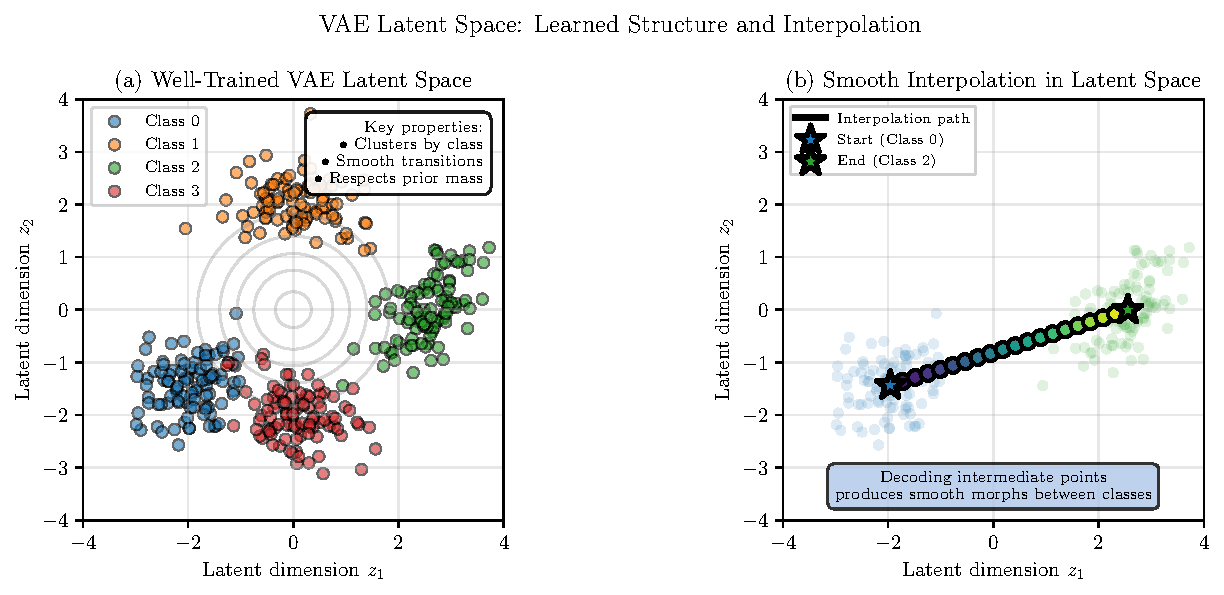
\includegraphics[width=\linewidth]{code/figures/ch08_variational_flows/fig_8_12_latent_structure.pdf}
\caption{Inspect latent structure: well-trained VAEs cluster related datapoints, assign higher KL usage to informative factors, and reveal traversals that modify interpretable attributes.}
\label{fig:latent_structure}
\end{figure}

\vspace{1.5em}

\subsection{Tighter Bounds: Importance Weighted Autoencoders}

The standard ELBO uses a single sample $z \sim q_\phi(z \mid x)$ to estimate the expectation. Importance weighted autoencoders (IWAE) use multiple samples and importance weighting to get a tighter bound:
%
\begin{equation}
\log p_\theta(x) \geq \mathbb{E}_{z_1, \ldots, z_K \sim q_\phi} \left[ \log \frac{1}{K} \sum_{k=1}^K \frac{p_\theta(x, z_k)}{q_\phi(z_k \mid x)} \right]
\end{equation}

\vspace{0.3cm}

This bound is tighter than the standard ELBO (which is the $K=1$ case) and approaches the true log-likelihood as $K \to \infty$. The cost is $K$ times more computation: we must evaluate the decoder and posterior for $K$ different $z$ samples.

\vspace{0.3cm}

IWAE is particularly useful when the approximation gap is large (the posterior family is not very flexible). It does not help with the amortization gap, however, and can sometimes exacerbate it by relying more heavily on the importance weights than on improving the posterior.

\vspace{2em}

%==========================
\section{Information Geometry: Projections and Flow Maps}
\label{sec:info_geometry}
%==========================

\vspace{1em}

\subsection{VAEs as I-Projections}

From an information-geometric perspective, variational inference performs an I-projection (information projection) of the true posterior onto the variational family. Minimizing $D_{\text{KL}}(q \| p)$ is mode-seeking: $q$ concentrates on regions where $p$ has high density, potentially ignoring other modes if the variational family cannot represent them simultaneously.

\vspace{0.3cm}

This is different from an M-projection (moment/mixture projection), which minimizes $D_{\text{KL}}(p \| q)$ and is mode-covering: $q$ spreads out to cover all of $p$'s modes, even if that means being diffuse.

\vspace{0.3cm}

The choice of direction matters. I-projections (KL(q || p)) are tractable because we can sample from $q$ and evaluate both $q$ and $p$. M-projections require expectations under $p$, which is often the hard part (that is why we are doing inference in the first place). But I-projections can miss important modes of the posterior, leading to underestimation of uncertainty.

\vspace{1.5em}

\begin{geometrylens}
In the space of probability distributions, the KL divergence defines a geometry where distances are measured by information. An I-projection finds the closest point in the variational family to the true posterior, where "closest" means minimum reverse KL $D_{\text{KL}}(q\|p)$. This projection respects the constraints of the family (e.g., diagonal covariance for mean-field) while trying to match the posterior as well as possible within those constraints. Geometrically, we are projecting onto a lower-dimensional manifold (the variational family) embedded in the space of all distributions.
\end{geometrylens}

\vspace{1.5em}

\begin{figure}[t]
\centering
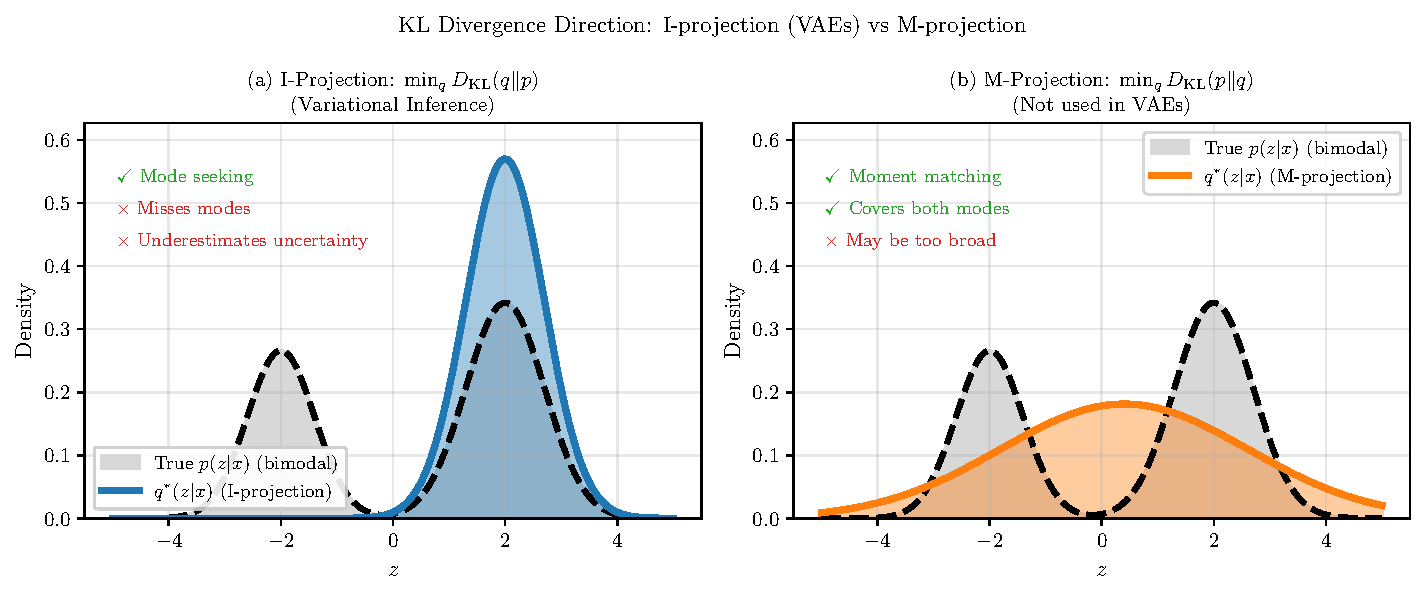
\includegraphics[width=\linewidth]{code/figures/ch08_variational_flows/fig_8_11_i_vs_m_projection.pdf}
\caption{I-projections minimize $D_{\mathrm{KL}}(q\|p)$ and hug high-density regions, while M-projections minimize $D_{\mathrm{KL}}(p\|q)$ and spread to cover all modes. Variational inference performs the former.}
\label{fig:i_vs_m_projection}
\end{figure}

\vspace{1.5em}

\subsection{Flows as Pushforward Maps}

Normalizing flows operate in a different geometric framework. Instead of projecting distributions, they define diffeomorphisms (smooth bijections) that push forward a simple base measure to the data distribution.

\vspace{0.3cm}

The geometry here is about how maps transform volumes and densities. The log-determinant term in the change-of-variables formula measures the local expansion or contraction of volume. A region of latent space with measure $\mu$ is mapped to a region of data space with measure $|\det J_f| \cdot \mu$.

\vspace{0.3cm}

Training a flow is optimizing the map $f$ to make the pushforward distribution $f_\sharp p_0$ match the data distribution. This is a different optimization objective than VAE training: we are directly shaping the generative map rather than approximating a posterior.

\vspace{0.3cm}

The geometric view helps us understand why certain architectures work. Coupling layers are partitioned maps that leave some dimensions unchanged while transforming others as a function of the fixed dimensions. This is geometrically special: it means the map is triangular in a particular coordinate system, making the determinant calculation trivial.

\vspace{1.5em}

\subsection{Complementary Perspectives on the Same Problem}

VAEs and flows solve the generative modeling problem from opposite directions. VAEs start with an inference question ("what latent $z$ explains data $x$?") and derive a generative model through variational approximation. Flows start with a transformation question ("how do we map noise to data?") and derive a density through change of variables.

\vspace{0.3cm}

These are not competing philosophies but complementary tools. Some problems are more naturally framed as inference (where we genuinely care about latent structure), others as transformation (where we just want to model density). Understanding both perspectives makes you a better modeler, able to choose the right tool and combine them when appropriate.

\vspace{2em}

%==========================
\section{Looking Forward}
\label{sec:looking_forward}
%==========================

\vspace{1em}

We have explored three paradigms for generative modeling with latent variables: variational inference with its ELBO objective, bits-back coding that reveals why the ELBO is exactly right for compression, and normalizing flows that avoid approximation through invertible maps. Each has distinctive strengths and weaknesses.

\vspace{0.3cm}

These models complement the autoregressive and diffusion models from earlier chapters. Autoregressive models excel at sequential structure and exact likelihood but lack compact latent representations. Diffusion models produce high-quality samples through iterative refinement but are slow and do not provide latent codes. VAEs compress data into interpretable latents but optimize bounds rather than exact objectives. Flows give exact likelihoods and invertibility but at computational cost.

\vspace{0.3cm}

The unifying thread is information geometry. Every model defines a trajectory through probability space: autoregressive models build distributions token by token, diffusion models flow from noise to data through score fields, VAEs project posteriors onto tractable families, flows push forward base measures through diffeomorphisms. Understanding these geometric perspectives helps us see connections between seemingly different approaches and design better architectures.

\vspace{0.3cm}

In the next chapters, we will see how these foundations extend to large-scale systems: training dynamics, scaling laws, and the peculiar geometry of overparameterized models. The ideas from this chapter---compression, calibration, amortization gaps---will reappear in new forms as we tackle the challenges of modern machine learning at scale.

\vspace{1em}

\begin{pausebox}
\textbf{Chapter Summary.} Variational autoencoders approximate intractable posteriors using the ELBO, which is both a likelihood lower bound and the expected codelength under bits-back coding (up to small overhead). The ELBO trades off reconstruction quality against prior matching, with three distinct gaps: approximation (family expressiveness), amortization (shared encoder), and optimization (training quality). Normalizing flows avoid approximation by using invertible maps with tractable Jacobians, providing exact likelihoods at the cost of architectural constraints. VAEs excel at learning compressed latent representations; flows excel at exact density modeling. Understanding both as different geometries on the space of distributions---I-projections versus pushforward maps---helps us choose the right tool and combine them effectively.
\end{pausebox}

\vspace{1.5em}

\section*{Exercises}
\begin{enumerate}
\item Derive the ELBO from the KL divergence between the approximate and true posterior. Show all steps explicitly.

\item For a Gaussian VAE where both prior and posterior are diagonal Gaussians, compute the closed form of the KL divergence.

\item Implement the reparameterization trick for a simple 2D VAE. Train it on synthetic data (mixture of Gaussians) and visualize the latent space.

\item Show that bits-back coding achieves expected codelength equal to $-\text{ELBO}$ by working through the encoding/decoding protocol step by step.

\item For a 2D coupling layer, write down the Jacobian matrix explicitly and verify that its determinant equals $\exp(\sum s_i)$.

\item Compare MAF and IAF: show concretely why MAF is fast for density evaluation and slow for sampling, and vice versa for IAF.

\item Implement KL annealing for a VAE on MNIST. Plot how the reconstruction loss, KL term, and sample quality evolve as the KL weight increases.

\item Measure the three gaps (approximation, amortization, optimization) on a trained VAE by: (a) using a more flexible posterior family, (b) doing per-example posterior refinement, (c) training longer. Which gap is largest?

\item (Hard) Derive the instantaneous change-of-variables formula for continuous normalizing flows. Start from the discrete-time change of variables and take the limit as $dt \to 0$.

\item Design a posterior predictive check for a VAE trained on a dataset of your choice. What statistics should match between real and generated data? Implement the check and report results.
\end{enumerate}

\vspace{2em}
